% !TeX spellcheck = en_GB
% !TeX program = pdflatex
%
% LuxSleek-CV 1.1 LaTeX template
% Author: Andreï V. Kostyrka, University of Luxembourg
%
% 1.1: added tracking and letter-spacing for prettier lower caps, added `~` for language levels
% 1.0: initial release
%
% This template fills the gap in the available variety of templates
% by proposing something that is not a custom class, not using any
% hard-coded settings deeply hidden in style files, and provides
% a handful of custom command definitions that are as transparent as it gets.
% Developed at the University of Luxembourg.
%
% *NOTHING IS HARCODED, and never should be.*
%
% Target audience: applicants in the IT industry, or business in general
%
% The main strength of this template is, it explicitly showcases how
% to break the flow of text to achieve the most flexible right alignment
% of dates for multiple configurations.

\documentclass[10pt, a4paper]{article} 

\usepackage[T1]{fontenc}     % We are using pdfLaTeX,
\usepackage[utf8]{inputenc}  % hence this preparation
\usepackage[british]{babel}  
\usepackage[left = 0mm, right = 0mm, top = 0mm, bottom = 0mm]{geometry}
\usepackage[stretch = 25, shrink = 25, tracking=true, letterspace=30]{microtype}  
\usepackage{graphicx}        % To insert pictures
\usepackage{marvosym}        % Provides icons for the contact details
\usepackage[dvipsnames]{xcolor}



\usepackage{enumitem}        % To redefine spacing in lists
\setlist{parsep = 0pt, topsep = 0pt, partopsep = 1pt, itemsep = 1pt, leftmargin = 6mm}

\usepackage[default]{FiraSans}     % Change this to use any font, but keep it simple
\renewcommand{\familydefault}{\sfdefault}

\definecolor{cvblue}{HTML}{304263}

%%%%%%% USER COMMAND DEFINITIONS %%%%%%%%%%%%%%%%%%%%%%%%%%%
% These are the real workhorses of this template
\newcommand{\dates}[1]{\hfill\mbox{\textbf{#1}}} % Bold stuff that doesn’t got broken into lines
\newcommand{\is}{\par\vskip.5ex plus .4ex} % Item spacing
\newcommand{\smaller}[1]{{\small$\diamond$\ #1}}
\newcommand{\headleft}[1]{\vspace*{3ex}\textsc{\textbf{#1}}\par%
    \vspace*{-1.5ex}\hrulefill\par\vspace*{0.7ex}}
\newcommand{\headright}[1]{\vspace*{2.5ex}\textsc{\Large\color{cvblue}#1}\par%
     \vspace*{-2ex}{\color{cvblue}\hrulefill}\par}
%%%%%%%%%%%%%%%%%%%%%%%%%%%%%%%%%%%%%%%%%%%%%%%%%%%%%%%%%%%%

\usepackage[colorlinks = true, urlcolor = gray,  linkcolor = gray]{hyperref}

\begin{document}

% Style definitions -- killing the unnecessary space and adding the skips explicitly
\setlength{\topskip}{0pt}
\setlength{\parindent}{0pt}
\setlength{\parskip}{0pt}
\setlength{\fboxsep}{0pt}
\pagestyle{empty}
\raggedbottom

\begin{minipage}[t]{0.33\textwidth} %% Left column -- outer definition
%  Left column -- top dark rectangle
\colorbox{cvblue}{\begin{minipage}[t][5mm][t]{\textwidth}\null\hfill\null\end{minipage}}

\vspace{-.2ex} % Eliminates the small gap
\colorbox{cvblue!90}{\color{white}  %% LEFT BOX
\kern0.09\textwidth\relax% Left margin provided explicitly
\begin{minipage}[t][293mm][t]{0.82\textwidth}
\raggedright
\vspace*{2.5ex}

\Large Susy \textbf{\textsc{Echeverria-Londono, PhD}} \normalsize \\
\emph{Consultante en recherche en biodiversité et santé publique. }

% Centering without extra vertical spacing
%\null\hfill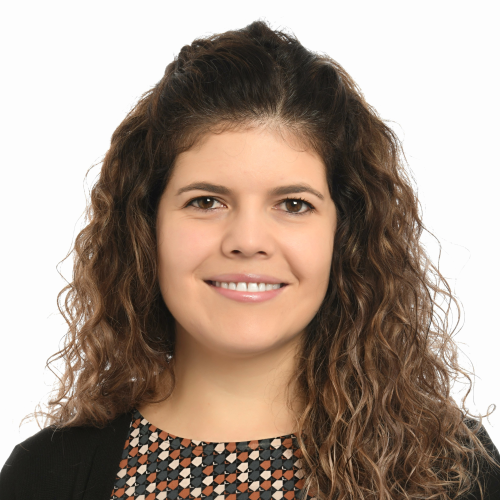
\includegraphics[width=0.65\textwidth]{Profile.png}\hfill\null

\headleft{Coordonnées}
\small % To fit more content
\MVAt\ {\small susyelo@gmail.com} \\[0.4ex]
\Mobilefone\ +33 6 36 01 15 45 \\[0.5ex]
\Mundus\ \href{https://susyelo.github.io/}{susyelo.github.io} \\[0.1ex]
\Letter\ Région parisienne, France
\normalsize

\headleft{Résumé professionnel}
\small Chercheuse pluridisciplinaire avec plus de 10 ans d’expérience à l’intersection de la biodiversité, de la santé publique et des sciences de l’environnement. Experte dans la synthèse et la communication de résultats scientifiques complexes à destination des chercheurs, décideurs politiques et grand public. Solides compétences en synthèse scientifique, visualisation de données et coordination collaborative à travers l’Europe, les Amériques et des consortiums internationaux (par ex. OMS, GAVI, NSF, VIMC).


\headleft{Compétences}
\normalsize

\begin{itemize}

\item Outils : R, Python, Git, Excel, LaTeX, Suite Office.
\item Multilingue (espagnol natif, anglais professionnel, français/italien intermédiaire).
\item Direction de projets de recherche internationaux et publications scientifiques (par ex. VIMC, financés par NSF)
\item Expérience dans la présentation et la rédaction de rapports pour des publics variés, incluant scientifiques, décideurs et grand public.
\item Solide expérience de travail avec des équipes internationales.
\item Expérience dans la coopération bilatérale et internationale (Amérique latine et Royaume-Uni).
\item Grande capacité à synthétiser des données complexes en informations accessibles.
\item Proactive et bien organisée, avec une forte capacité à prioriser et un bon esprit d’équipe.

\end{itemize} 

\headleft{Centres d’intérêt}
En dehors du travail, je pratique la danse, je profite de promenades régulières avec mon chien et ma famille.


\end{minipage}%
\kern0.09\textwidth\relax%%Right margin provided explicitly to stretch the colourbox
}
\end{minipage}% Right column
\hskip2.5em% Left margin for the white area
\begin{minipage}[t]{0.56\textwidth}
\setlength{\parskip}{0.8ex}% Adds spaces between paragraphs; use \\ to add new lines without this space. Shrink this amount to fit more data vertically

\vspace{2ex}

\headright{Formation}
\small
\textsc{\textbf{Doctorat (Ph.D.)} en Sciences de la Vie}  \dates{2013--2017} \\
 \textit{Imperial College London, Royaume-Uni}.\\
\smaller{\textit{Thèse : Macrovévolution des plantes et réponses de la biodiversité aux changements d’utilisation des terres.}}

\is
\textsc{\textbf{Master Recherche} (M.Res.)} en Biodiversité, Informatique et Génomique  avec distinction \dates{2012--2013} \\
\textit{Imperial College London, Royaume-Uni}.  \\
\smaller{Thèse : Effets de l’usage des terres sur la biodiversité locale en Colombie.}

\is
\textsc{\textbf{Licence en Biologie}} (mention très bien)  \dates{2004--2010} \\
\textit{Universidad Industrial de Santander, Colombie}. 


\headright{Expérience professionnelle}

\is
\textsc{Consultante en recherche (freelance)} \dates{2022-- aujourd’hui}  \\  
\textit{Global / Télétravail}   \\
{\small \begin{itemize}
	\item Soutien aux institutions de politique publique dans l’évaluation du potentiel d’harmonisation et d’intégration des estimations d’impact vaccinal à travers plusieurs plateformes.
  	\item Communication des résultats à travers des rapports destinés à des parties prenantes mondiales (VIMC, GAVI et BMGF).
\end{itemize}}
        		
\is	
\textsc{Consultante et Associée de recherche}    \dates{2019--2022} \\
\textit{Imperial College London, Royaume-Uni} \\
{\small  \begin{itemize}     
  	\item Collaboration avec une équipe multidisciplinaire de chercheurs, d’experts techniques, d’organisations axées sur les politiques et de chefs de projet pour produire des rapports de recherche et d’orientation politique.
  	\item Production de livrables robustes et pertinents pour les politiques de santé mondiale ; rédaction régulière de rapports techniques pour soutenir la prise de décision fondée sur des données probantes.
  	\item Rédaction de notes de synthèse et de rapports pour appuyer les décisions stratégiques en matière de vaccination à l’échelle mondiale.
  	\item Collaboration avec des chercheurs colombiens pour comprendre la propagation et l’évolution initiale du SARS-CoV-2 en Colombie.
\end{itemize}}

\is
\textsc{Chercheuse postdoctoral (NSF)}  \dates{2017--2019} \\
\textit{Kenyon College, Ohio, États-Unis} \\
{\small \begin{itemize}
	\item Direction de recherches sur la biodiversité végétale à travers différents biomes en Amérique, intégrant des données phylogénétiques et écologiques.
	\item Co-développement et enseignement d’un module international “Écologie globale et biogéographie”.
 	\item Collaboration avec des chercheurs brésiliens sur l’évolution des biomes. \textit{PIs : Prof. Andrew Kerkhoff et Prof. Brian J. Enquist}
\end{itemize} }

\is  
\textsc{Chargée de cours et démonstratrice} \dates{2013--2017} \\  
\textit{Muséum d’Histoire Naturelle / Imperial College London, Royaume-Uni} \\
{\small \begin{itemize}
  	\item Coordination de la collecte et de l’analyse de données sur le terrain entre chercheurs colombiens et institutions britanniques.
  	\item Contribution à la diplomatie scientifique de haut niveau, présentation des résultats de recherche à des personnalités comme le président colombien, des ministres et le prince Charles.
\end{itemize} }

\headright{Projets et Réalisations}
\small
\begin{itemize}
\item Gestion de la livraison hebdomadaire de rapports destinés à l’OMS, GAVI, et BMGF, en respectant des délais stricts.
\item Coordination de la collecte de données et de la communication entre chercheurs colombiens et européens pour des projets de suivi de biodiversité (ex. : PREDICTS).
\item Plus de 30 articles dans des revues à comité de lecture (Lancet, Nature, eLife, Vaccine): \url{https://susyelo.github.io/publications.html}
\item Lauréat du prix "Outstanding Paper by Young Investigator" (JSE, 2022).
\end{itemize}

\end{minipage}

\begin{minipage}[t][293mm][t]{0.82\textwidth}

\end{minipage}%
\hskip2.5em% Left margin for the white area
\begin{minipage}[t]{0.9\textwidth}

\setlength{\parskip}{0.8ex}% Adds spaces between paragraphs; use \\ to add new lines without this space. Shrink this amount to fit more data vertically

\headright{Biodiversity Publications}
\small

\begin{itemize}
\setlength\itemsep{0.6em}

\item 2021. Neves, D.M., Kerkhoff, A.J., \textbf{Echeverr\'ia-Londo\~no, S,.}  Merow, C., Morueta-Holme, N., Peet, R.K., Sandel, B., Svenning, J.C., Wiser, S.K. and Enquist, B.J.  The adaptive challenge of extreme conditions shapes evolutionary diversity of plant assemblages at continental scales, \textit{Proceedings of the National Academy of Sciences} 118(37).\url{https://doi.org/10.1073/pnas.202113211}

\item 2020. \textbf{Echeverr\'ia-Londo\~no, S,.}  S{\"a}rkinen, T., Fenton, I. S., Knapp, S. and Purvis, A. Dynamism and context dependency in the diversification of the megadiverse plant genus Solanum L. (Solanaceae), \textit{Journal of Systematics and Evolution},  58(6), 767-782. \url{https://doi.org/10.1111/jse.12638}

\item 2018. \textbf{Echeverr\'ia-Londo\~no, S.,} Enquist. B. J., Neves, D. M., Violle, C. and Kerkhoff, A. J. Plant functional diversity and the biogeography of biomes in North and South America. \textit{Frontiers in Ecology and Evolution}, 6(DEC), 219. \url{https://doi.org/10.3389/fevo.2018.00219}

\item 2017. Isaacs, P., \textbf{Echeverr\'ia-Londo\~no, S.,} Urbina, N. and Purvis, A. Species composition and changes in land use: considerations under climatic change scenarios. Moreno, L. A., Andrade, G. I. and Ru\'iz-Contreras, L. F. (Editors). In \textit{Biodiversity 2016. Status and Trends of Colombian Continental Biodiversity}, Instituto de Investigaci\'on de Recursos Biol\'ogicos Alexander von Humboldt, 106 p. \url{http://reporte.humboldt.org.co/biodiversity/2016/cap2/203/index.html}

\item 2017. Hudson, L. N., Newbold, T., Contu, S., Hill, S. L., Lysenko, I., De Palma, A., Diaz, S., \textbf{Echeverr\'ia-Londo\~no, S.,} \dots and Purvis, A. The database of the PREDICTS (Projecting Responses of Ecological Diversity in Changing Terrestrial Systems) project, \textit{Ecology and Evolution}, 7(1), 145--188. \url{https://doi.org/10.1002/ece3.2579}

\item 2016. \textbf{Echeverr\'ia-Londo\~no, S.,} Newbold, T., Hudson, L. N., Hill, S. L., Contu, S., Lysenko, I., \dots and Purvis, A. Modelling and projecting the response of Colombian biodiversity to land-use change, \textit{Diversity and Distributions}, 22, 1099--1111. \url{https://doi.org/10.1111/ddi.12478}

\item 2015. Newbold, T., Hudson, L. N., Hill, S. L., Contu, S., Lysenko, I., Senior, R. A., Bennet D. J., Choimes A., Collen, B., Day, J., De Palma, A., Diaz, S., \textbf{Echeverr\'ia-Londo\~no, S.,} \dots and Purvis, A. Global effects of land use on local terrestrial biodiversity, \textit{Nature}, 520(7545), 45--50. \url{https://doi.org/10.1038/nature14324}

\item 2014 . Newbold, T., Hudson, L. N., Contu, S.,  Hill, S. L., Lysenko, I., De Palma, A., Phillips, H., Senior, R. A., Bennet D. J., Booth, H., Choimes, A., Correia, D. L. P., Day, J., \textbf{Echeverr\'ia-Londo\~no, S.,} \dots and Purvis, A. The PREDICTS database: a global database of how local terrestrial biodiversity responds to human impacts, \textit{Ecology and Evolution}, 4(24), 4701--4735. \url{https://doi.org/10.1002/ece3.1303}

\item 2011 . \textbf{Echeverr\'ia-Londo\~no, S.} and Miranda-Esquivel, D. R. MartiTracks: A geometrical approach for identifying geographical patterns of distribution, \textit{PLoS ONE}, 6(4), e18460. \url{https://doi.org/10.1371/journal.pone.0018460}

\end{itemize}

\headright{Public Health Publications}

\small

\begin{itemize}
\setlength\itemsep{0.6em}

\item 2024. Hartner, A. M., Li, X., \textbf{Echeverr\'ia-Londo\~no, S,.}  Roth, J., Abbas, K., Auzenbergs, M., ... \& Gaythorpe, K. A. (2024). Estimating the health effects of COVID-19-related immunisation disruptions in 112 countries during 2020–30: a modelling study. The Lancet Global Health, 12(4), e563-e571.

\item 2023. Hartner, A. M., Li, X., \textbf{Echeverr\'ia-Londo\~no, S,.} Roth, J., Abbas, K., Auzenbergs, M., ... \& Gaythorpe, K. COVID-19 Related Immunisation Disruptions from 2020-2030: Projecting Health Impact and Mitigation Strategies for 14 Pathogens Across 112 Low- and Middle-Income Countries. \url{http://dx.doi.org/10.2139/ssrn.4492698}

\item 2022. Ali, H.A., Hartner, AM., \textbf{Echeverr\'ia-Londo\~no, S,.}. \& et al. Vaccine equity in low and middle-income countries: a systematic review and meta-analysis. \textit{Int J Equity Health} 21, 82. \url{https://doi.org/10.1186/s12939-022-01678-5}

\item 2022. \textbf{Echeverr\'ia-Londo\~no, S,.}  Hartner, A. M., Li, X., Roth, J., Portnoy, A., Sbarra, A. N., ... \& Gaythorpe, K. A. Exploring the subnational inequality and heterogeneity of the impact of routine measles immunisation in Africa. \textit{Vaccine}, 40(47), 6806-6817. \url{https://doi.org/10.1016/j.vaccine.2022.09.049}

\item 2022. Toor, J., Li, X., Jit, M., Trotter, C. L., \textbf{Echeverr\'ia-Londo\~no, S,.}  Hartner, A. M., ... \& Gaythorpe, K. A. COVID-19 impact on routine immunisations for vaccine-preventable diseases: Projecting the effect of different routes to recovery. \textit{Vaccine}, 40(31), 4142-4149. \url{https://doi.org/10.1016/j.vaccine.2022.05.074}

\item 2022. Ali, H.A., Hartner, AM., \textbf{Echeverr\'ia-Londo\~no, S,.}  et al. Vaccine equity in low and middle-income countries: a systematic review and meta-analysis. \textit{Int J Equity Health} 21, 82.\url{ https://doi.org/10.1186/s12939-022-01678-5}

\item 2021. \textbf{Echeverr\'ia-Londo\~no, S,.}  Li, X., Toor, J., de-Villiers, M., Nayagam, S., Hallett, T.B., Abbas, K., Jit, M., Klepac, P., Jean, K. \&  Garske, T. How can the public health impact of vaccination be estimated? \textit{BMC Public Health}, 21, 2049 (2021). \url{https://doi.org/10.1186/s12889-021-12040-9}

\item 2021. Toor, J., \textbf{Echeverr\'ia-Londo\~no, S,.} Li, X., Abbas, K., Carter, E. D., Clapham, H. E., ... \& Gaythorpe, K. A. Lives saved with vaccination for 10 pathogens across 112 countries in a pre-COVID-19 world, \textit{eLife} 10, e67635.\url{https://doi.org/10.7554/eLife.67635}

\item 2021. Gaythorpe, K. A., Toor, J., \textbf{Echeverr\'ia-Londo\~no, S,.}  Li, X., \& Ferguson, N. M. Vaccines can save children with non-preventable diseases Authors' reply.  Estimating the health impact of vaccination against ten pathogens in 98 low-income and middle-income countries from 2000 to 2030: a modelling study, \textit{The Lancet} 397(10291), 2251. \url{https://doi.org/10.1016/S0140-6736(21)01015-1}

\item2021. Li, X., Mukandavire, C., Cucunub\'a, Z. M., \textbf{Echeverr\'ia-Londo\~no, S,.} Abbas, K., Clapham, H. E., ... \& et al.  Estimating the health impact of vaccination against ten pathogens in 98 low-income and middle-income countries from 2000 to 2030: a modelling study, \textit{The Lancet},  397(10272), 398-408. \url{https://doi.org/10.1016/S0140-6736(20)32657-X}

\item 2021. Gaythorpe K, Abbas K, Huber J, Karachaliou A, Thakkar N, Woodruff K, Li X, \textbf{Echeverr\'ia-Londo\~no, S,.}  Ferrari M, Jackson ML, McCarthy K. Impact of COVID-19-related disruptions to measles, meningococcal A, and yellow fever vaccination in 10 countries, \textit{eLife}, 2021;10:e67023. \url{https://doi.org/10.7554/elife.67023}

\item 2020. Laiton-Donato, K., Villabona-Arenas, CJ., Usme-Ciro, J.,  Franco-Mu\~noz., C,  \'Alvarez-D\'iaz, D., Villabona-Arenas, LS., \textbf{Echeverr\'ia-Londo\~no, S,.} et al.,  Genomic epidemiology of severe acute respiratory syndrome coronavirus 2, Colombia, \textit{Emerging infectious diseases},  26, no. 12: 2854. \url{https://doi.org/10.3201/eid2612.202969}

\end{itemize}

\end{minipage}

\end{document}